\chapter{Preliminary Experiments}

\section{Dataset}
In our work we use the TIGER dataset which was released with the challenge under the same name on the Grand Challenge platform \cite{tiger_dataset}. It contains H\&E stained WSIs of Her2 positive and TNBC breast cancer tissues obtained by core needle biopsies or surgical resections. The size of a single pixel equals approximately 0.5 \textmu m on all images. The dataset is released in three formats. We work with the one called WSIROIS. The WSIs come from three different institutions:

\begin{enumerate}
    \item TCGA (151 WSIs) dataset, contains images of TNBC from the TCGA-BRCA archive, annotations and magnification was adopted to be in-line with those used further.
    \item RUMC (26 WSIs) images of both TNBC and Her2 positive breast cancer obtained from Radbound University Medical Centre in Netherlands, annotated by a panel of board-certified pathologists.
    \item JB (18 WSIs) images of both TNBC and Her2 positive breast cancer obtained from Jules Bordet Institute in Belgium, annotated by a panel of board-certified pathologists.
\end{enumerate}

The RUMC and JB WSIs contain 3 annotated ROIs with a size of approximately $500\!\times\!500$ \textmu m. The WSIs obtained from TCGA are more specific. This dataset was created by merging two other datasets: the BCSS (151 WSIs) and the NuCLS (124 WSIs). The NuCLS is a subset of the BCSS dataset. In the BCSS dataset the tissue in a single large ROI is annotated but no cells are annotated. In the NuCLS a variable number of smaller ROIs are selected within the large ROI (same large ROI as in the BCSS) and these are densely annotated for multiple cell types. Annotations are adopted to match the other used annotations, as was mentioned.

The WSIROIS format contains:

\begin{itemize}
    \item WSI level annotations, where in each WSI contains manual annotations of ROIs. Different tissue types are annotated with polygons, namely: invasive tumor, tumor-associated stroma, in-situ tumor, healthy glands, necrosis not in-situ, inflamed stroma, rest. Most ROIs have also annotated plasma cells and lymphocytes. These were annotated using point annotations and then a bounding box was constructed and centred on the point of annotation with size of $8\!\times\!8$ \textmu m. Annotations for WSIs are released in XML format and also as a multi-resolution TIF image.
    \item ROI level annotations, where authors cropped the ROIs from WSIs and stored them as PNG files. Tissue type annotations are released as PNG images, containing pixel-level masks and cell annotations are released in the COCO format - a JSON file containing file paths (the PNG images of ROIs) with IDs and metadata and corresponding annotations of bounding box position and size.
\end{itemize}

We further work with the part of dataset that has ROI level annotations. This part of dataset consists of 1,879 (1,744 from TCGA, 81 from RUMC, 54 from JB) ROIs cropped from 44 (124 from TCGA, 26 from RUMC, 18 from JB). Together they contain 30,524 annotated cell nuclei.

\section{Experiments}
So far our experiments mostly contained the data preprocessing step, where we downloaded the dataset, explored it and made sure we can load the images and annotations for visual assessment and initial overview. All of the experiments were done on a personal notebook, MacBook Air with M1 chip and 16 GB of RAM. We use the Python programming language, version 3.12 in the PyCharm IDE. For the image preprocessing we utilize the Open CV library. We use Git as a version control system and GitHub as a remote repository, where we periodically save progress.

\subsection{Dataset Loading and Project Structure}
Since the images in our dataset are in PNG format, it is easy to load them with the Open CV Python library functions as well as the Pillow (successor of the Python Imaging Library - PIL) library functions. The annotations of the TIL cells are in JSON format and can be effortlessly loaded with the Python built-in module for handling this type of files.

The project file structure can be seen in figure \ref{fig:project-structure}.

\begin{figure}[H]
    \begin{centering}
    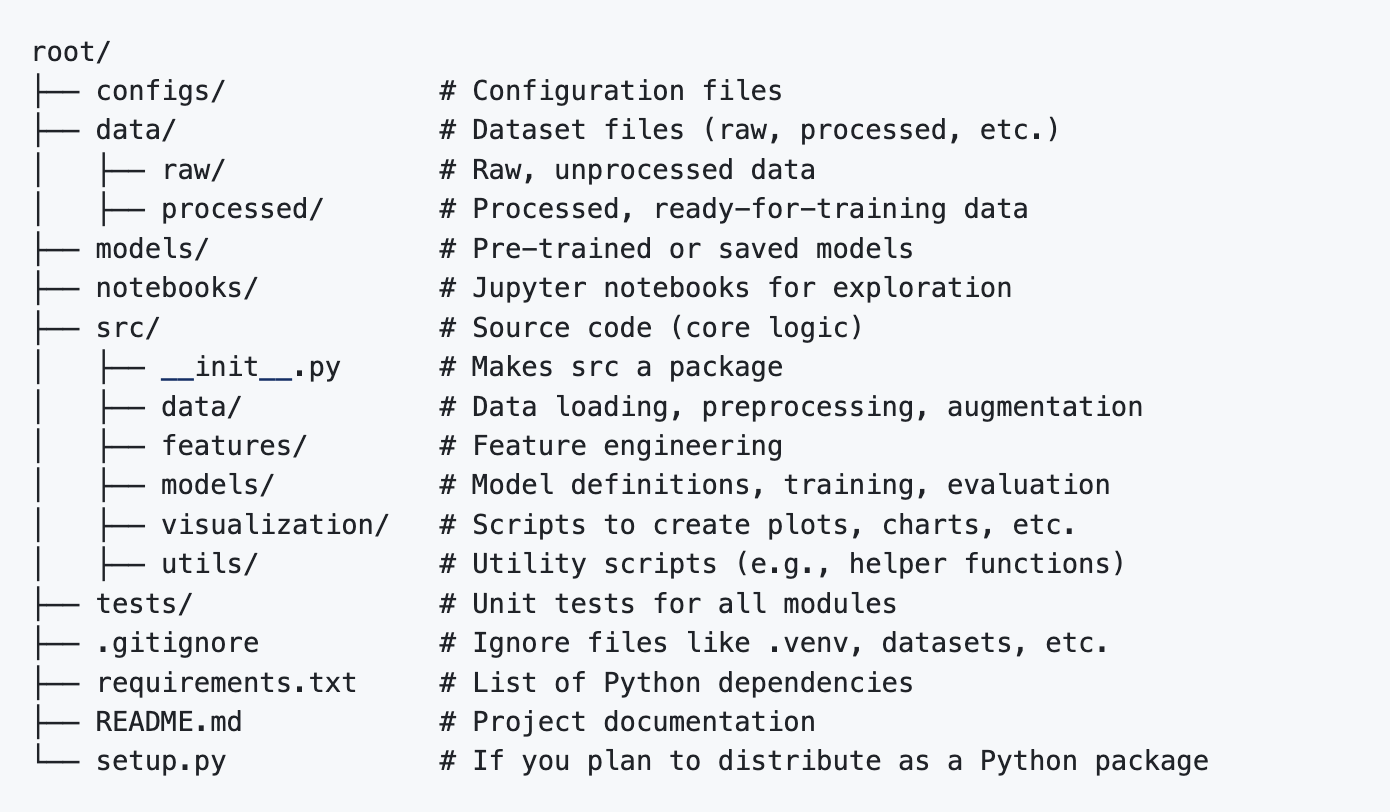
\includegraphics[width=14cm]{assets/images/project-structure.png}
    \par\end{centering}
    \caption{The proposed project file structure}
    \label{fig:project-structure}
\end{figure}

\subsection{Normalization Experiments}
Since the images come from different datasets, institutions, and surgical procedures (core needle biopsies, surgical resections), we applied a Macenko normalization to all H\&E stained images with a random image selected as a reference image. The visual result can be seen in figure \ref{}. As we can see, this caused the images were shifted into the purple-like colours. We considered other approaches to select a reference image, but as recent study \cite{Ivanov2024} showed, than when selecting only a single reference image the results will always be biased and suboptimal. Therefore we would like to try experimenting with their proposed method of selecting multiple images to obtain better results. We would also like to try the normalization method used in \cite{Vahadane2015}, which showed promising results.

\subsection{Single-cell Cropping}
Next preprocessing step involved cropping out single cell from the larger PNG image. Since the location and size of each cell's bounding box was provided within the JSON file, the cells were easily cropped out using a simple Python script. The visual procedure of cropping out the cells from normalized images can be seen in figure \ref{}.

\subsection{GrabCut Experiments}
We use these single-cell images as an input for the GrabCut algorithm provided by the Open CV library. In this step we wanted to create the pseudo-labels for the cells, which could be used further to train a deep learning model. We experimented with different combinations of normalized/non-normalized images, tried to apply the power law (gamma) transformation to the images and Contrast Limited Adaptive Histogram Equalization (CLAHE) method with varying parameters as well. We also experimented with different number of pixels that were set as sure background as a GrabCut parameter, for example we let $N$ brightest pixels be the sure background (since cell nuclei are coloured by haematoxylin into deep purple and blue colours, while the tissue and cellular matrix is coloured into more bright red and pink tones). 

The best visual result we obtained can be seen in figure \ref{}. It was done on the normalized images, with applied CLAHE (clip limit was set to 100 and tile grid size to (1,1)) and 100 brightest pixels ($\frac{100}{256} = 0.390625 = 39.0625\%$ of image pixels) set as sure background to GrabCut. As we can see from the figure \ref{}, although the resulting masks look promising they are still far from ideal, especially in images where there is lower contrast between the cell nuclei and surrounding area. This challenge needs to be addressed in the next phase of work. We mention different methods for obtaining pseudo-label masks we want to experiment with in the former chapter \ref{chap-solution-concept}. 